\chapter{Pendulum}
After succeeding to generate simple, interpretable solutions for cart-pole and mountain-car, I wanted to choose an environment that (1) was similar enough to expect the same general approach to be fruitful, and (2) posed a challenge that the GP algorithm had not yet overcome. Pendulum (also known as the inverted pendulum problem) is another popular classic control RL benchmark that simulates a pendulum suspended from a frictionless pivot. In the initial state of the environment the angle of the pendulum is randomised. The goal is to swing it until it points upwards and then keep it steady for as long as possible. Interestingly, the mechanics of the problem are very similar to mountain-car, but with one important difference that makes it significantly more difficult to solve: the desired state of the environment (the pendulum pointing up, which is equivalent to the car standing on top of the hill) needs to, not only be reached, but maintained. Practically, this means that the agent has to combine two strategies: one for transitioning to that desired state and another one for maintaining it.

%%%%%%%%%%%%%%%%%%%%%%%%%%%
% 6.1 Environment Details %
%%%%%%%%%%%%%%%%%%%%%%%%%%%
\section{Environment Details}
The observation object for this environment consists of the trigonometric functions $sin(\theta)$ (\verb+sintheta+) and $cos(\theta)$ (\verb+costheta+), which on a high level describe the angle between the pendulum and the horizontal axis, and the angular velocity of the pendulum, $\dot\theta$ (\verb+thetadot+) which is a measure of how fast the pendulum is rotating. The sign of \verb+thetadot+ indicates whether the pendulum is rotating clockwise (negative) or anticlockwise (positive), while the signs of \verb+costheta+ and \verb+sintheta+ vary based on the spatial region the pendulum occupies. Notice that this allows for the environment space to be split into four quadrants based on the signs of these two quantities (figure \ref{fig:pendulum_quadrants}), an observation that proved very useful in conceptualising many aspects of the problem and interpreting the various solutions the algorithm generated. The action space is the range $[-2.0, 2.0]$ of floating-point numbers, which represent the force (torque) that is applied to control the pendulum's rotation. Finally, the reward comes in the form of a cost, which means the agent receives a negative reward at each time-step (the maximum is $0$) that is proportional to the angle of the pendulum, its angular velocity, and the torque applied to it (see the GitHub Wiki page\footnote{\url{https://github.com/openai/gym/wiki/Pendulum-v0}} for the precise equation for the reward). 

Therefore, the goal of the environment is to bring the pendulum to a vertical angle, and keep it there with minimum effort. Unlike the previous environments, the solution criteria here are unspecified, so the average reward of an agent that takes random actions ($\approx-1220$) was used as a reference point for measuring performance.

\begin{figure}[ht]
    \centering
    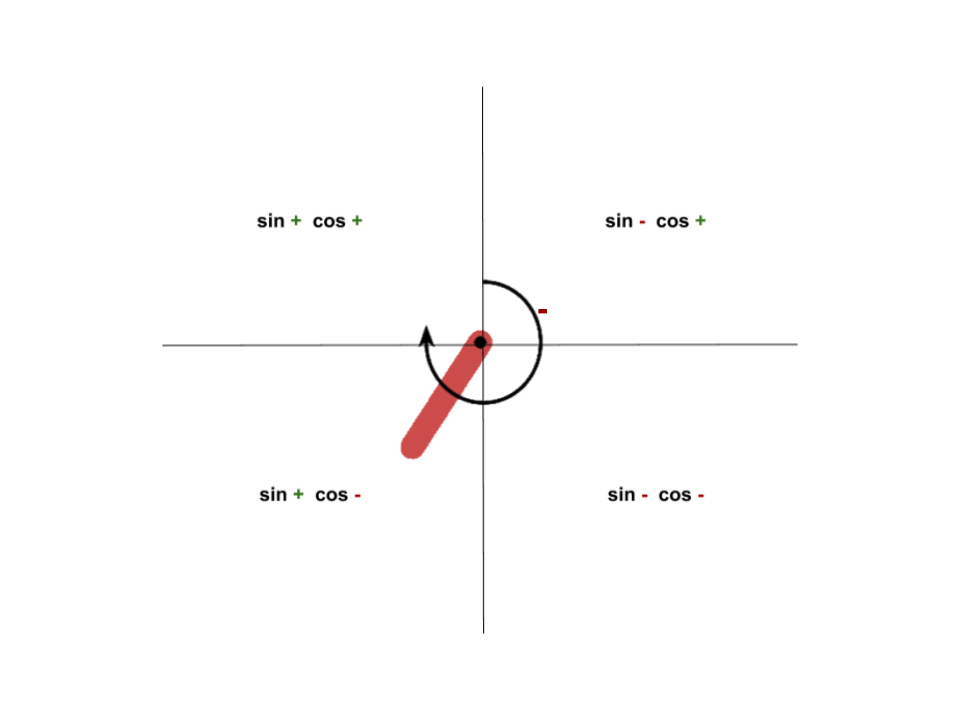
\includegraphics[width=12cm]{images/pendulum_quadrants.png}
    \caption{Visualisation of the signs of the pendulum observations}
    \label{fig:pendulum_quadrants}
\end{figure}

%%%%%%%%%%%%%%%%%%%%%%%%%%%%%%%%%%%%%
% 6.2 Experiment 1: Simple GP Agent %
%%%%%%%%%%%%%%%%%%%%%%%%%%%%%%%%%%%%%
\section{Experiment 1: Simple GP Agent}

% Setup %
\subsection{Setup and Motivation}
The main aim of the first experiment was to establish a performance baseline for the succeeding experiments to use as a reference point. Therefore, the program structure was simple, and similar to the one used in the previous environments:

\begin{verbatim}
F = {IFLTE}
T = {costheta, sintheta, thetadot, -1.0, 0.0, 1.0}
\end{verbatim}

The function set only includes the \verb+IFLTE+ function that proved very useful in solving the first two environments, and the terminal set includes all of the environment observations as well as three constants. The motivation behind the specific choice of constants was to allow the agent to draw decision boundaries around the observations (e.g. \verb+if costheta <= 0.0 and sintheta <= 0.0 then ...+) because a good strategy will probably need to make different decisions based on the angle of the pendulum. Since \verb+costheta+ and \verb+sintheta+ range over $[-1.0, 1.0]$, those limits were chosen as the constants, along with $0$ because it is reasonable to hypothesise that information about the sign of the observations is useful (for example the sign of \verb+thetadot+ can be used to determine whether the pendulum is rotating clockwise or anticlockwise).

The setup for this first experiment (summarised in table \ref{tab:pendulum_exp1_params}) followed that of the previous environments, with a few notable differences. Tournament selection was chosen instead of fitness proportionate selection, as discussed in Methods. Mutation was used for the first time to encourage exploration and avoid early convergence, both of which were not necessary in cart-pole and mountain-car. Notice, also, that while in the previous environments the terminal fitness was always the average reward required for a solution, the value used here was chosen more arbitrarily since pendulum has no specified solution criterion. Additionally, since pendulum has no episode termination criteria, the episode length had to be constrained explicitly. Finally, the number of episodes each program was run for to compute its fitness had to be decreased. The reason for this was, again, the absence of termination criteria: in cart-pole and mountain-car, even though the maximum episode length was 200 time-steps, most episodes did not run for that long, especially during the first few generations, because the programs failed quickly, causing the episodes to terminate prematurely. In pendulum, however, no such restriction exists, which meant that every program ran for the full episode length every time. As a result, the training time significantly increased, and it became impractical to run multiple experiments. The solution of reducing the number of episodes came at the cost of robustness because the fitness of each program became more sensitive to the randomisation of the initial environment state. This cost did not seem to be severe, however, since the experiment results showed a steady improvement in overall fitness from generation to generation. 

\begin{table}[ht]
    \centering
    \begin{tabular}{|l|c|}
        \hline
        \textbf{Parameters} & \textbf{Values} \\
        \hline
        Population size     & 200  \\
        Max generations     & 20   \\
        Terminal fitness & -200 \\
        Tournament size     & 10   \\
        Mutation rate       & 0.1  \\
        Max program depth   & 5    \\
        Number of runs      & 10   \\
        Number of episodes  & 10   \\
        Episode length      & 200  \\
        \hline
    \end{tabular}
    \caption{Experimental parameters (Pendulum Experiment 1)}
    \label{tab:pendulum_exp1_params}
\end{table}

% Results %
\subsection{Results and Discussion}
\subsubsection{Average Fitness Per Generation}
The average fitness the programs of each generation achieved is visualised in figure \ref{fig:pendulum_exp1_plot}. The first generation of programs performed very poorly, which was expected since they were randomly generated, but performance radically improved during the first four generations, before converging and remaining roughly the same for the remainder of the GP run. While the GP algorithm performed as expected, with each generation of programs performing better than the previous ones, it converged on a sub-optimal solution very quickly and showed no sign of improvement thereafter. Increasing the mutation rate delayed convergence and increased the variance in average fitness, but failed to make the algorithm escape the local minimum it appeared to be stuck on. These results gave rise to the hypothesis that the algorithm had discovered the best possible strategy given its current program structure, and failed to find a better solution because the program space was too restricted. Therefore, it was decided that the next experiment would introduce additional features to the language that could potentially be used to discover better solutions.

\begin{figure}[ht]
    \centering
    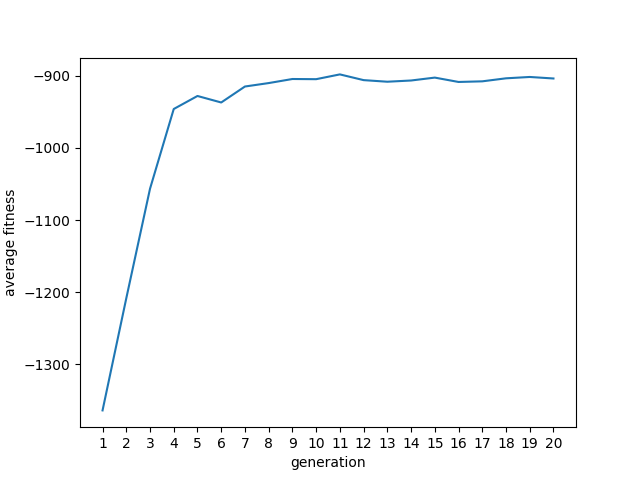
\includegraphics[width=12cm]{images/pend_simple_gp_agent.png}
    \caption{Average population fitness vs generations}
    \label{fig:pendulum_exp1_plot}
\end{figure}

\subsubsection{Best-Performing Programs}
At the end of each of the 10 runs of GP, the best-performing program, as well as the average reward (fitness) it achieved over 100 consecutive episodes, were recorded. The average fitness achieved by these programs was $-857$ and the programs themselves can be seen in table \ref{tab:pendulum_exp1_best_programs}. Looking at these programs, it quickly becomes obvious that most of them are identical or logically equivalent to the program \verb+IFLTE(thetadot, 0.0, costheta, 0.0)+. Additionally, it turned out that the programs that seem to be different due to their complexity (programs 3, 5, and 8 in the table) can also be reduced to this program. Therefore, the algorithm did not simply converge on various strategies with similar performance scores, but on syntactically equivalent programs that encoded a single strategy. This observation provided further evidence that the hypothesis regarding the limitations imposed by the program structure was correct.

\begin{table}[ht]
    \centering
    \begin{tabular}{|l|c|}
        \hline
        \multicolumn{1}{|c|}{\textbf{Programs}} & \textbf{Fitness} \\
        \hline
        
        \verb+IFLTE(thetadot, 0.0, costheta, 0.0)+ & -906  \\ \hline
        \verb+IFLTE(0.0, thetadot, 0.0, costheta)+ & -835  \\ \hline
        \verb+IFLTE(0.0, IFLTE(-1.0, 1.0, thetadot, sintheta), 0.0, costheta)+ & -884  \\ \hline
        \verb+IFLTE(thetadot, 0.0, costheta, 0.0)+ & -826  \\ \hline
        
        \verb+IFLTE(thetadot, 0.0, costheta,+ & \\
        \verb+  IFLTE(IFLTE(1.0, thetadot,+ & -833 \\
        \verb+  IFLTE(-1.0, 0.0, -1.0, thetadot), -1.0), -1.0, 0.0, thetadot))+ & \\
        \hline
        
        \verb+IFLTE(0.0, thetadot, 0.0, costheta)+ & -852  \\ \hline
        \verb+IFLTE(0.0, thetadot, 0.0, costheta)+ & -832  \\ \hline
        
        \verb+IFLTE(0.0, thetadot,IFLTE(costheta, 1.0,+ & \\
        \verb+  IFLTE(0.0, 1.0, 0.0, costheta),+ & -892 \\
        \verb+  IFLTE(0.0, -1.0, costheta, -1.0)), costheta)+ & \\
        \hline
        
        \verb+IFLTE(thetadot, 0.0, costheta, 0.0)+ & -868  \\ \hline
        \verb+IFLTE(0.0, thetadot, 0.0, costheta)+ & -842  \\ \hline
    \end{tabular}
    \caption{Best programs of each GP run (Pendulum Experiment 1)}
    \label{tab:pendulum_exp1_best_programs}
\end{table}

\subsubsection{Strategy Interpretation}
The program discovered by the GP algorithm, while not optimal, performed significantly better than a random agent, which made it a good starting point for tackling pendulum. It is, therefore, useful to discuss the interpretation of the strategy this program encodes to identify its limitations and justify the improvements implemented in the subsequent experiments. As noted in the environment description, the agent's goal is twofold: swing the pendulum until it's standing upright, and then keep it there with minimum effort. So, the strategy should be examined in terms of how well (or poorly) it performs with respect to these two sub-goals. 

The strategy encoded by this program is: "if the pendulum is rotating clockwise (negative angular velocity), then apply a torque to it that is equal to the cosine of its angle; otherwise, apply no torque to it at all." To understand this strategy, one needs to understand how \verb+costheta+ changes in the environment. As seen in figure \ref{fig:pendulum_quadrants}, \verb+costheta+ is negative in the bottom two quadrants, $0$ when the pendulum is parallel to the horizontal axis, and positive in the upper two quadrants. Therefore, concerning the first sub-goal, if the pendulum is rotating clockwise, a negative torque is applied to it, accelerating its clockwise rotation, whereas if the pendulum is rotating anticlockwise, it is let to swing freely. The result of this is that the pendulum is repeatedly pushed to rotate clockwise, then allowed to swing back freely, until it has built enough momentum to swing to the upper section of the screen. An interesting detail to note is that as the pendulum approaches a horizontal angle from the bottom quadrants, \verb+costheta+, and in turn the applied torque, tend to $0$. The effect of this is that the pendulum's momentum is great enough for it to reach an upright position, but not too great to cause it to be impossible to slow down (and, then, balance) once it has reached it. Finally, notice that this first half of the strategy is similar to the one discovered for mountain-car, where the car is pushed back-and-forth until it has enough momentum to climb the hill and reach the goal. This makes sense considering the similarity between the two environments discussed earlier.

It is clear that this strategy achieves the first sub-goal, but the difference to mountain-car is that the agent now has to use a different strategy to achieve the additional sub-goal of balancing the pendulum upright. When the pendulum enters the top-left quadrant, \verb+costheta+ becomes positive. Since \verb+thetadot+ is still negative at this point, this change causes the pendulum to slow down, as an opposite torque equal to \verb+costheta+ is applied to it. When \verb+thetadot+ is decreased to $0$ the else-branch of the if-statement encoded in the strategy takes effect and no torque is applied, preventing the pendulum to enter an anticlockwise rotation. The observed result is that the pendulum gradually slows down until it reaches the vertical position, then begins to speed up as it reaches the upper-right quadrant, and eventually falls to the bottom, letting the entire process repeat, with the only difference being that the pendulum has enough momentum now to not need to be swung back-and-forth to 'escape' the bottom quadrants.

\subsubsection{Problems and Ideas For Improvement}
This strategy solves the first sub-problem of escaping the bottom quadrants adequately and approximates a solution to the second sub-problem of keeping the pendulum standing upright by slowing it down and then applying no torque to it, which keeps it close to a vertical angle for some time and minimises the applied effort. The issue with this strategy is that, while the pendulum slows down, it doesn't stop once it reaches that vertical angle, so it inevitably falls to one side and keeps rotating.

It seemed that the current program structure should be sufficient to figure out an improvement for this strategy that addressed this issue. For example, a nested if-statement might be used to describe a new case where the pendulum is at a vertical angle and an action to take in that case, which would result in the desirable balancing behaviour. Additionally, as discussed above, it was reasonable to assume, based on the results, that the algorithm suffered from an early convergence problem that an extension to the program space might be able to improve. With this in mind, the second experiment was set up with a minor extension to the program structure and an encouragement of exploration in the form of an increase to the program depth and the maximum number of generations to evolve.

%%%%%%%%%%%%%%%%%%%%%%%%%%%%%%%%%
% 6.3 Experiment 2: Exploration %
%%%%%%%%%%%%%%%%%%%%%%%%%%%%%%%%%
\section{Experiment 2: Exploration}

% Setup %
\subsection{Setup and Motivation}
This experiment was intentionally very similar to experiment 1. As seen in table \ref{tab:pendulum_exp2_params}, most parameters were left unchanged with a few exceptions. Specifically, the terminal fitness was decreased from $-200$ to the theoretical maximum, $0$, in case this version of the agent managed to find an exceptionally good solution. More importantly, the maximum number of generations and the program depth were increased to encourage exploration by allowing the GP algorithm more time to generate more complex programs.

The program structure was also very similar, with only two additions that would hopefully allow for better strategies to emerge without reducing interpretability. The function \verb+neg+, which simply returns the opposite of a numerical input, was introduced to increase the number of combinations of observation values used without introducing completely new constructs. Secondly, a small constant ($0.25$) was added to the terminal set to give the agent an alternative value to use as an action. The motivation behind this last addition was that if one of the evolved strategies managed to balance the pendulum at a vertical angle, it would need to apply as small a torque as possible to minimise its effort. Finally, the constants $1.0$ and $-1.0$ were removed, since they didn't prove to be useful in the previous experiment.

\begin{table}[ht]
    \centering
    \begin{tabular}{|l|c|}
        \hline
        \textbf{Parameters} & \textbf{Values} \\
        \hline
        Population size     & 200  \\
        Max generations     & 30   \\
        Terminal fitness & 0 \\
        Tournament size     & 10   \\
        Mutation rate       & 0.1  \\
        Max program depth   & 10    \\
        Number of runs      & 5   \\
        Number of episodes  & 10   \\
        Episode length      & 200  \\
        \hline
    \end{tabular}
    \caption{Experimental parameters (Pendulum Experiment 1)}
    \label{tab:pendulum_exp2_params}
\end{table}

% Results %
\subsection{Results \& Discussion}
\subsubsection{Average Fitness Per Generation}
As seen in figure \ref{fig:pendulum_exp2_plot}, the average fitness followed a similar pattern to that of the previous experiment, starting very low and increasing rapidly in the first 4 generations. However, in this case, the algorithm did not converge on a single strategy at that point, but kept improving for the remainder of the run. This is an indication that expanding the program space had the desired effect of allowing the algorithm to escape the sub-optimal solution it was stuck on and discover better-performing strategies.

\begin{figure}[ht]
    \centering
    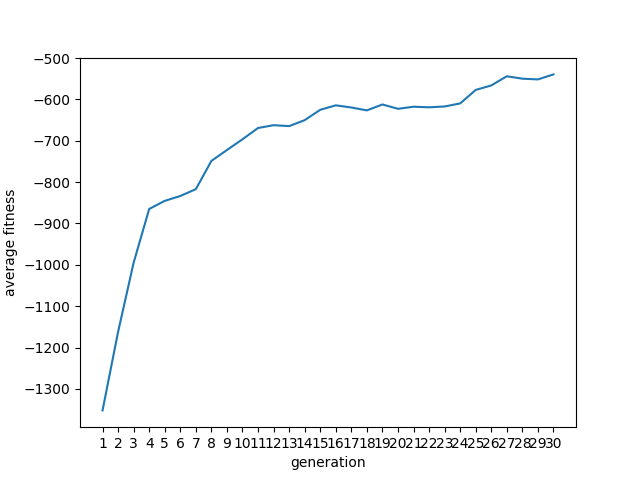
\includegraphics[width=12cm]{images/pendulum_deep_simple_GP.png}
    \caption{Average population fitness vs generations}
    \label{fig:pendulum_exp2_plot}
\end{figure}

\subsubsection{Best-Performing Programs}
While already visible in the average fitness graph, the best-performing programs of each GP run confirmed that the experiment was a success. The 5 generated programs, listed in table \ref{tab:pendulum_exp2_best_programs}, achieved an average fitness score of $-494.8$, almost half of what was achieved in the previous experiment, without an increase in complexity. Additionally, similarly to the previous experiment, all of these programs encode a single strategy which is easy to interpret. It is also interesting to note that the only useful modification to the program structure seems to have been the introduction of the \verb+neg+ function. Finally, increasing the population size and the number of maximum generations did not yield a better strategy, which is an indication that the algorithm had once again reached the limits allowed by the current program structure, so an improvement would probably require a language extension.

\begin{table}[ht]
    \centering
    \begin{tabular}{|l|c|}
        \hline
        \multicolumn{1}{|c|}{\textbf{Programs}} & \textbf{Fitness} \\
        \hline
        
        \verb+IFLTE(neg(sintheta), thetadot, neg(costheta), costheta)+ & -550  \\ \hline
        \verb+IFLTE(neg(sintheta), thetadot, neg(costheta), costheta)+ & -453  \\ \hline
        \verb+IFLTE(thetadot, neg(sintheta), costheta, neg(costheta))+ & -522  \\ \hline
        \verb+IFLTE(neg(thetadot), sintheta, neg(costheta), costheta)+ & -480  \\ \hline
        
        \verb+IFLTE(thetadot, IFLTE(0.25, 0.0,+ & \\
        \verb+  thetadot, neg(sintheta)), costheta,+ & -469 \\
        \verb+  IFLTE(costheta, costheta, neg(costheta), neg(0.0)))+ & \\
        \hline
    \end{tabular}
    \caption{Best programs of each GP run (Pendulum Experiment 2)}
    \label{tab:pendulum_exp2_best_programs}
\end{table}

\subsubsection{Strategy Interpretation}
All of the programs generated by the GP algorithm are identical or logically equivalent to the program \verb+IFLTE(thetadot, neg(sintheta), costheta, neg(costheta))+, which encodes the following strategy: "if \verb+thetadot+ $\leq$ -\verb+sintheta+ then apply a torque of magnitude \verb+costheta+; otherwise, apply a torque of magnitude -\verb+costheta+." Due to the mathematical nature of the description of the environment, this strategy does not seem intuitively interpretable. It is, therefore, useful to examine how this strategy causes the pendulum to behave in each of the four quadrants, as displayed in figure \ref{fig:pendulum_quadrants}. Additionally, it is useful to assess how well this strategy performs with respect to the two sub-goals that the agent needs to achieve: (1) rotate the pendulum until it reaches an upward vertical angle and (2) keep the pendulum balanced once it reaches that position.

With respect to (1), the two bottom quadrants are of interest. If the pendulum is in the bottom-right quadrant and \verb+thetadot+ $\leq$ \verb+-sintheta+ then \verb+thetadot+ is in $[-8.0, 1.0]$, which means the pendulum is either rotating clockwise, or it's rotating anticlockwise at a very low speed. In this case, the strategy applies a torque of magnitude \verb+costheta+, which is a negative value. If, however, the pendulum is in the bottom-right quadrant and is rotating anticlockwise at a high speed, apply a torque of magnitude \verb+-costheta+, which is a positive value. Therefore, in the bottom-right quadrant, the strategy says, if the pendulum is rotating clockwise, or anticlockwise but at a low speed, then push it clockwise, but if it's rotating anticlockwise at a high speed, then push it anticlockwise. This seems to be the most efficient way of making the pendulum swing up to the top quadrants, so this part of the strategy is reasonable. 

If the pendulum is in the bottom-left quadrant, a similar rule is applied. If \verb+thetadot+ $\leq$ -\verb+sintheta+ then \verb+thetadot+ is in $[-8.0, 0.0]$, which means the pendulum is rotating clockwise. In this case, the pendulum is pushed by \verb+costheta+, and therefore clockwise since \verb+costheta+ is negative, accelerating its current rotation so that it can reach the top quadrants. If \verb+thetadot+ $\geq$ -\verb+sintheta+ then \verb+thetadot+ is in [-1.0, 8.0], which means it's rotating anticlockwise or clockwise at a low speed. In this case, the pendulum is pushed by -\verb+costheta+, and therefore anticlockwise, which also accelerates its current rotation. Again, this seems to be the most efficient way to increase the pendulum's momentum enough to make it escape the bottom quadrants and achieve the first sub-goal.

With respect to (2), the top quadrants are considered. If the pendulum is in the top-left quadrant and \verb+thetadot+ $\leq$ -\verb+sintheta+ then the pendulum is rotating clockwise. In this case, the pendulum is pushed by \verb+costheta+, and therefore anticlockwise. This serves to slow the pendulum down, which is the desired behaviour here. If the pendulum is in the top-left quadrant and rotating anticlockwise, then it's pushed clockwise, bringing it towards the desired vertical angle. Similarly, in the top-right quadrant, if the pendulum is rotating clockwise (or anticlockwise but at a very low speed) then it is pushed anticlockwise, which pushes it towards the vertical angle, and if it is rotating anticlockwise, then it is pushed clockwise, which slows it down.

\section{Manual Improvement}
\subsection{Problem With Current Strategy}
The strategy generated as a result of experiment 2, seemed to behave effectively with respect to both sub-goals, in each of the four states (quadrants) that the pendulum might be in. This, then, begged the question, why this strategy could not achieve a better score. The first possible problem (confirmed by manual observation) was that the maximum value of \verb+costheta+ and -\verb+costheta+ (the two values used as the applied torque) were not large enough to slow down the pendulum when it was swung up to the top quadrants. So, if the agent failed to balance the pendulum on its first rotation, it would have accumulated too much momentum by the second rotation for the agent to be able to slow down and balance it. 

\subsection{Manual Intervention and Significance of Results}
This problem seemed simple to address: every occurrence of \verb+costheta+ could be replaced with \verb+costheta+ multiplied by some constant, to increase the torque applied to the pendulum, which would hopefully allow it to maintain its balance once it has reached a vertical angle. To test this hypothesis, a simple, brute-force optimisation procedure was implemented, which evaluated the strategy multiple times, each time multiplying \verb+costheta+ by a different constant (the range used was $[1.0, 10.0]$), and returned the constant that made the strategy perform the best. The result was surprisingly positive. The same strategy, modified to multiply the applied torque by $9.0$, consistently achieved an average reward of $\approx-200$ over 100 consecutive episodes. For comparison, the best neural-network-based solutions on the environment leaderboard page\footnote{\url{https://github.com/openai/gym/wiki/Leaderboard}} achieve an average reward of $\approx-123$. The following is the program that achieved this result: \\\verb+IFLTE(thetadot, neg(sintheta), costheta*9.0, neg(costheta*9.0))+.

This result was very significant because it is evidence of the potential benefits of interpretable solutions to RL problems. The only way to improve a neural network is by adjusting its parameters or architecture and re-training it. However, this case study is a good example of how interpretability can be useful because it allows manual intervention via logic and intuition to systematically modify and improve the solutions discovered automatically by algorithms. 

\subsection{Further Problems and Future Extensions}
A second problem that was identified was that, once the agent had managed to balance the pendulum, it put too much effort (torque) into keeping it balanced, so it accumulated a lot of negative reward. So, an improvement to this strategy could involve a nested if-statement that is used to detect when the pendulum has been stabilised at a vertical position, and then reduce the applied torque to a minimum. Such an improvement would probably require an extension to the program structure and quite a bit of exploration using the GP algorithm to discover a program that encodes this behaviour. 
